\documentclass{beamer}
\usepackage{minted}
\setbeamertemplate{caption}{\raggedright\insertcaption\par}
\newcommand\Fontvi{\fontsize{9.5}{7.2}\selectfont}
\usepackage[T1]{fontenc}
\begin{document}

\title{Analisi della sicurezza binaria di WebAssembly}
\author{Alessandro Arata}
\institute{Universitá di Genova}
\date{\today}

\begin{frame}
  \titlepage
\end{frame}

\begin{frame}
  \frametitle{WebAssembly}
  \begin{columns}
    \begin{column}{0.6\textwidth}
      \begin{itemize}
        \item è un \textbf{target di compilazione}
        \begin{itemize}
          \item esistono compilatori da C(++), Rust ed altri linguaggi
        \end{itemize}
      \item è pensato per eseguire codice sui \textbf{browser} (recentemente anche su Node.js)

        \item è un linguaggio bytecode che offre tempi di esecuzione rapidi e un
        formato portabile e compatto
        \item è implementato dalla maggior parte dei browser
      \end{itemize}
    \end{column}
    \begin{column}{0.4\textwidth}
      \centerline{
\includegraphics[width=4cm,height=5cm,keepaspectratio]{images/logo.png}}
    \end{column}
  \end{columns}
\end{frame}

\begin{frame}
  \frametitle{WebAssembly - organizzazione di un programma}
  \begin{columns}
    \Fontvi
    \begin{column}{0.6\textwidth}
  \begin{itemize}
    \item le istruzioni sono eseguite su una \textbf{macchina virtuale} stack-based
    \item gli elementi del programma (per esempio funzioni o variabili) sono
      identificati da \textbf{indici} interi
    \begin{itemize}
      \item esistono sezioni che associano ad un indice una funzione o il
        valore di una variabile 
    \end{itemize}
    \item staticamente tipato con quattro tipi primitivi: 
      \begin{itemize}
        \item \textbf{i32} e \textbf{i64} per interi a 32 e 64 bit
        \item \textbf{f32} e \textbf{f64} per floating point a singola e doppia precisione
      \end{itemize}
    \item tipi complessi (stringhe, indirizzi, classi, struct...) vengono
      salvati in un'area di memoria chiamata \textbf{memoria lineare}
    \item lo stack delle chiamate e le variabili (globali o locali) di tipo
      primitivo sono gestiti dalla macchina virtuale
    \item la memoria lineare è gestita dal programma
  \end{itemize} 
  \end{column}
    \begin{column}{0.4\textwidth}
  \centerline{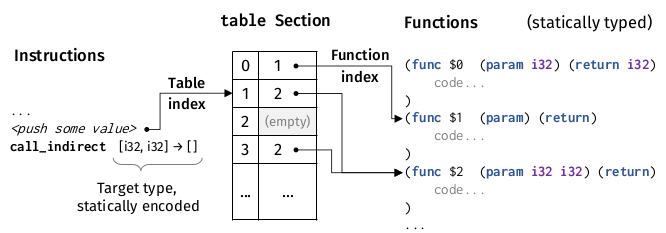
\includegraphics[width=5cm,height=5cm,keepaspectratio]{images/ftable.png}}
  \newline\newline\newline\newline
  \centerline{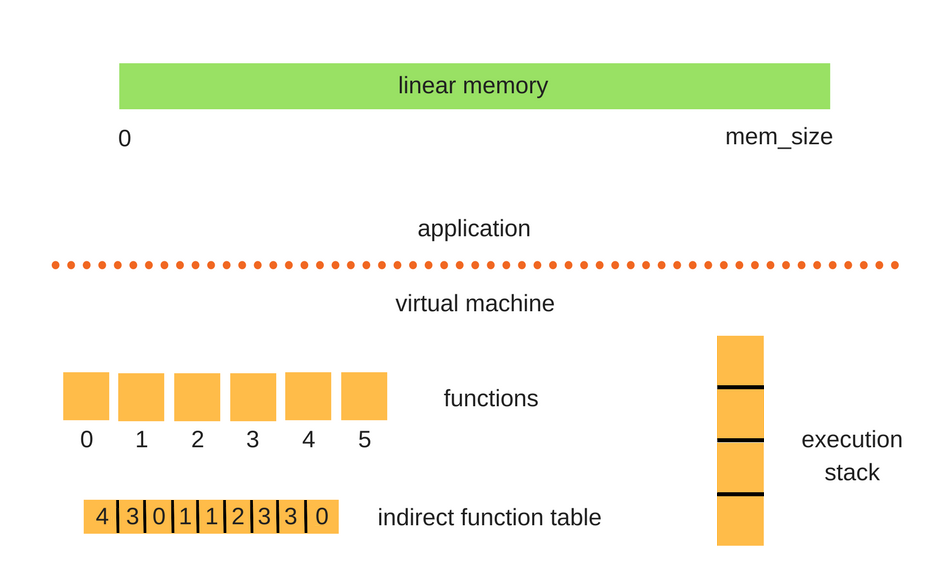
\includegraphics[width=10cm,height=3.5cm,keepaspectratio]{images/linmem.png}}
    \end{column}
  \end{columns}
\end{frame}

\begin{frame}[fragile]
  \frametitle{helloWorld.wat}
  \Fontvi
  \begin{minted}{c}
    puts("Hello, world!");
  \end{minted}

  viene compilato in 

  \begin{minted}{wat}
    (module
      ;; Imports from JavaScript namespace and log function
      (import  "console"  "log" (func  $log (param  i32  i32)))
      ;; Import 1 page of memory
      (import  "js"  "mem" (memory  1))
      ;; Data section of our module
      (data (i32.const 0) "Hello, world!")
      ;; Function declaration: Exported as helloWorld(), no arguments
      (func (export  "helloWorld")
        ;; pass offset 0 to log
        i32.const 0
        ;; pass length 13 to log (strlen of sample text)
        i32.const 13          
        call  $log
      )
    ) 
  \end{minted}
\end{frame}

\begin{frame}
  \frametitle{Memoria lineare}
  \begin{itemize}
    \item array \textbf{globale} di byte indirizzato da puntatori
    \begin{itemize}
      \item per indirizzare la memoria si utilizzano indici di tipo i32
    \end{itemize}
  \item è divisa in \textbf{regioni} per heap, stack e dati statici
    \item contiene tipi non primitivi 
    \item è sia leggibile che scrivibile ma non eseguibile 
    \item è totalmente allocata: ogni puntatore compreso tra [0, mem\_max]
      è valido 
  \end{itemize}

  \centerline{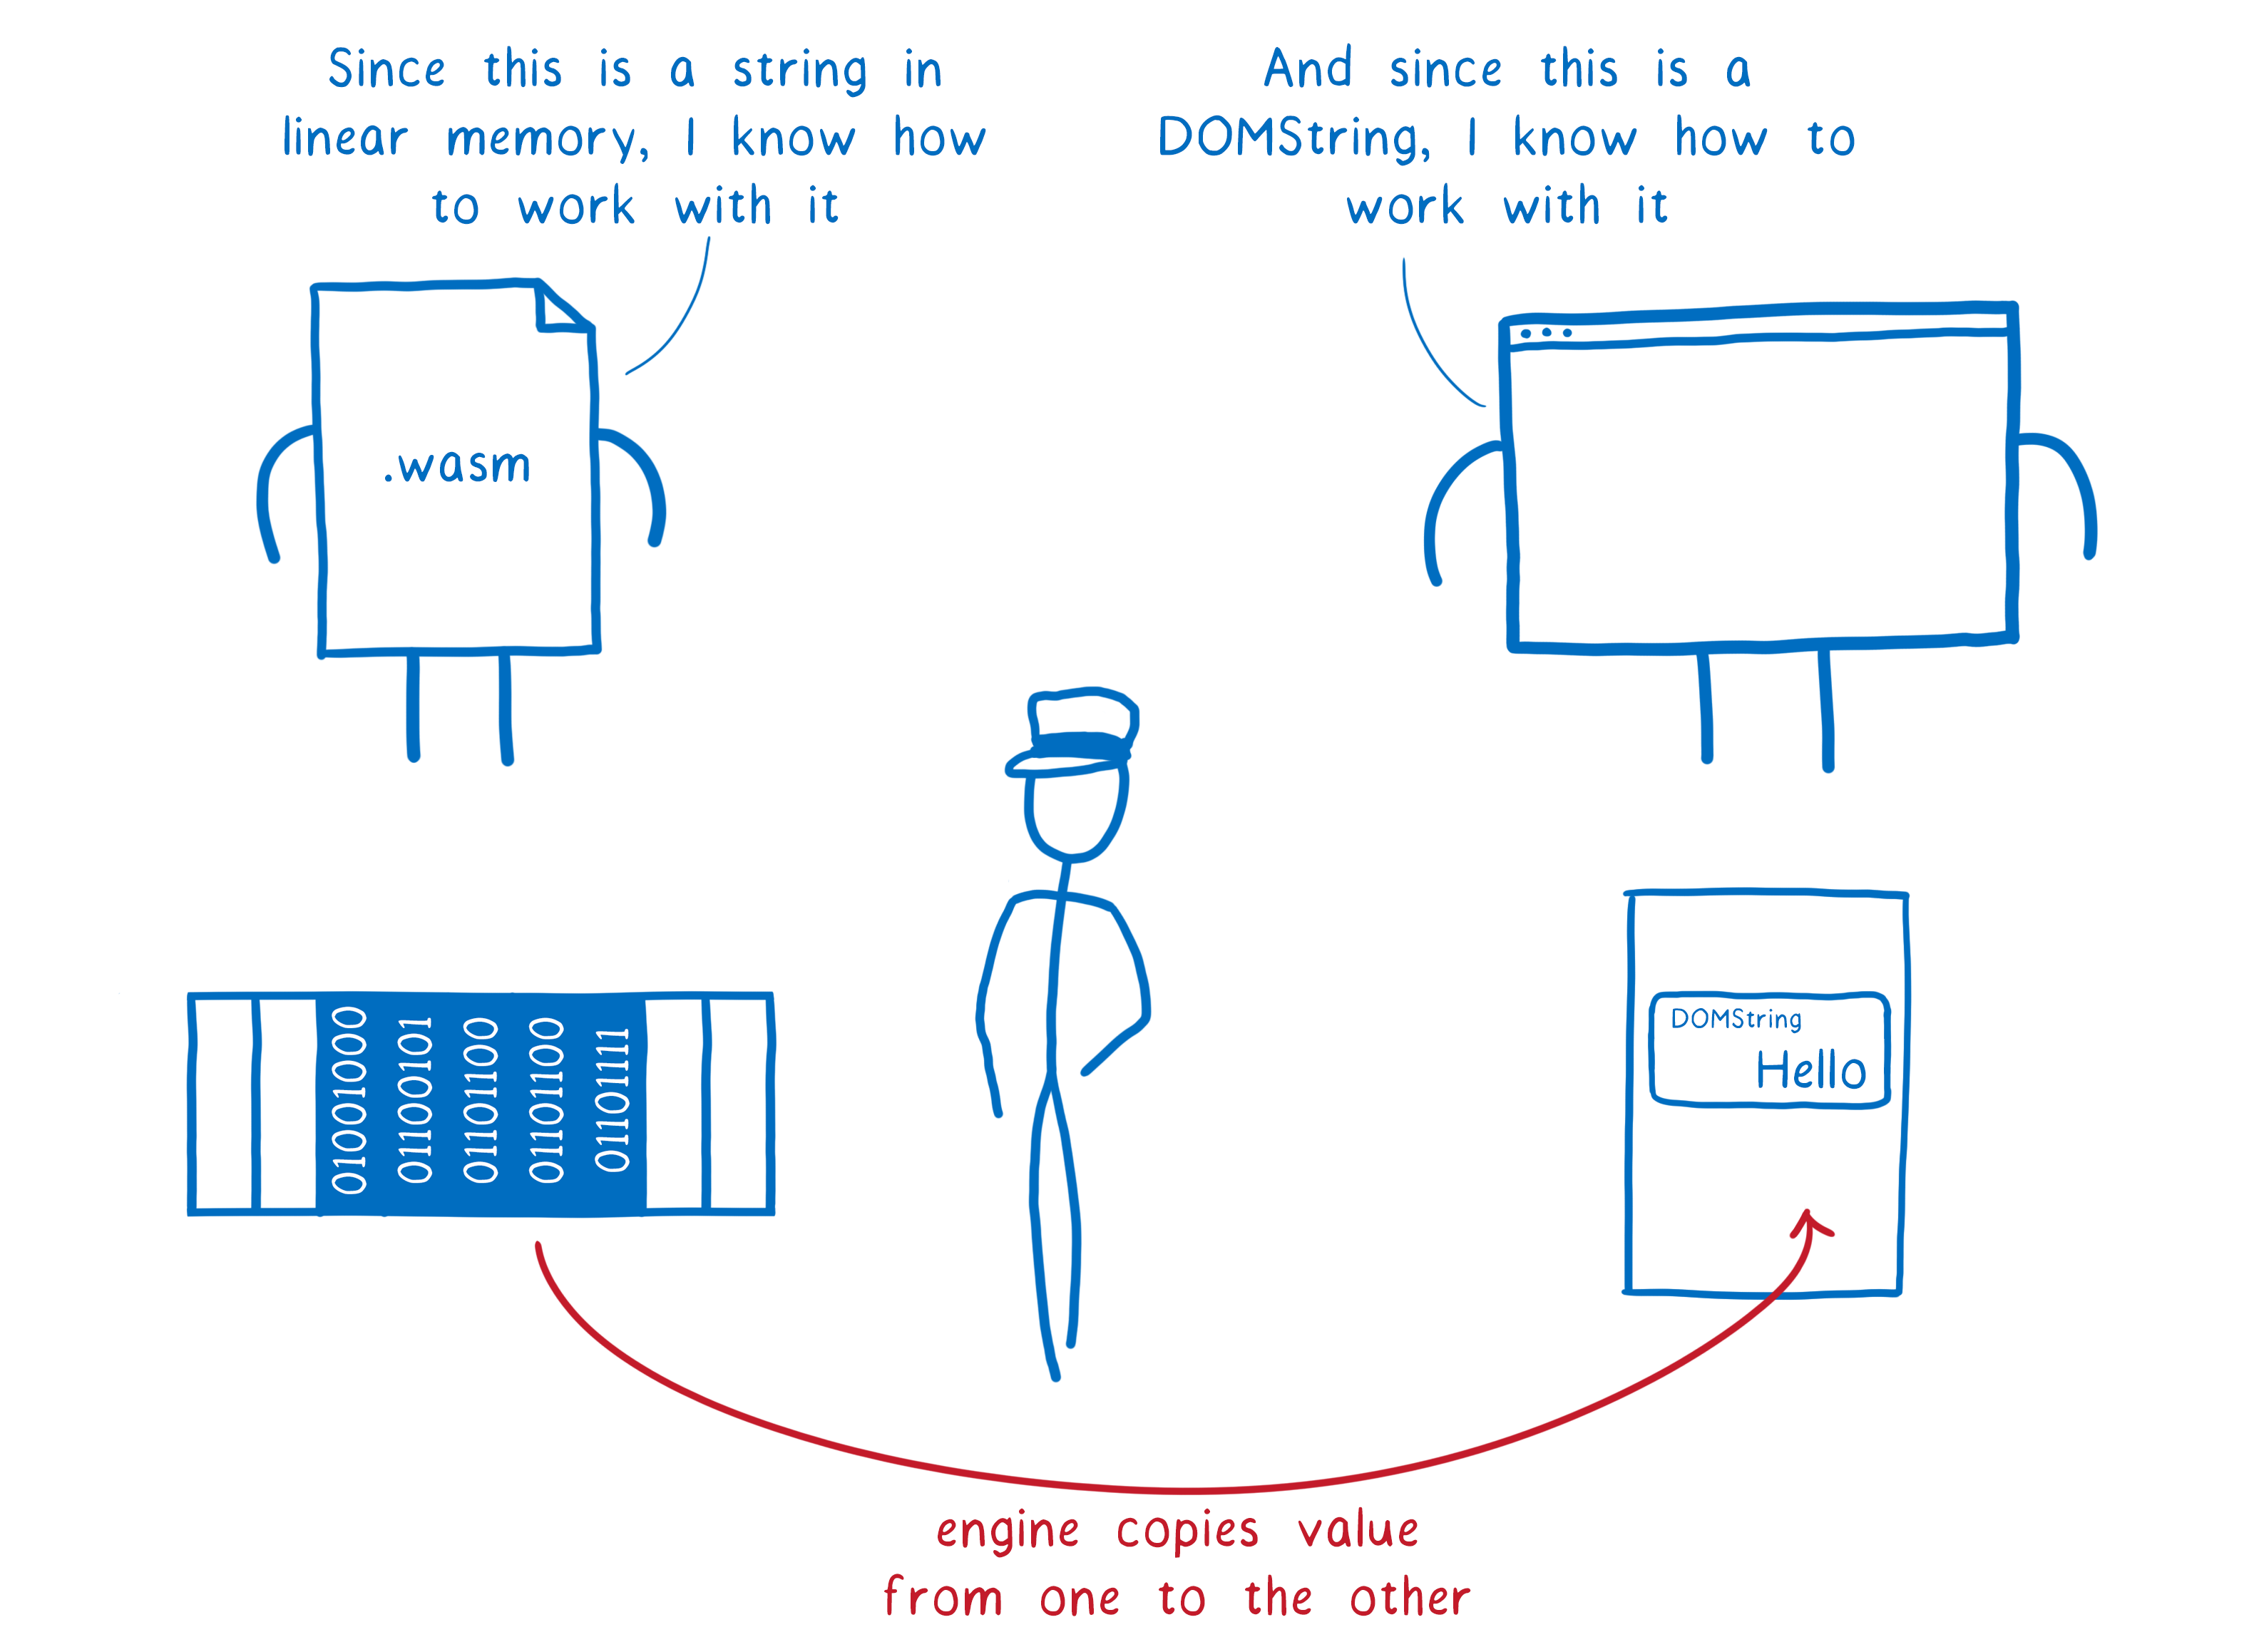
\includegraphics[width=10cm,height=5cm,keepaspectratio]{images/memman.png}}
\end{frame}

\begin{frame}
  \frametitle{Principali mitigazioni}
  \begin{itemize}
    \item i binari nativi offrono diverse mitigazioni in maniera da rendere
      difficile l'utilizzo di exploit della memoria
      \begin{itemize}
        \item \textbf{Address Layout Space Randomization} (ASLR): gli indirizzi
          del codice, dello stack e dello heap vengono modificati per ogni
          esecuzione
        \item \textbf{Guard page}: vengono inserite pagine non mappate tra le
          regioni della memoria (codice, stack e heap) per evitare che un
          overflow in una regione possa sovrascrivere dati in un'altra
        \item \textbf{Stack canary}: è un valore inserito prima dell'indirizzo di
          ritorno di una funzione; se il valore del canarino risulta diverso
          (a causa di un overflow) il programma viene interrotto  
      \end{itemize}
    \item esistono sezioni dedicate per i dati costanti e statici in modo che
      non possano essere sovrascritti
    \item la memoria del processo è divisa in pagine e possono non trovarsi tutte
      in memoria in un preciso momento dell'esecuzione
      \begin{itemize}
        \item un attaccante deve evitare di accedere a pagine non allocate
          (viene sollevato un fault)
      \end{itemize}
  \end{itemize}
\end{frame}

\begin{frame}
  \frametitle{Memoria lineare - sicurezza binaria}
  \begin{itemize}
    \item no \textbf{ASLR}: la posizione di una elemento è "predicibile" (dal
      compilatore utilizzato e dal programma)
    \item nessuna \textbf{guard page} tra le regioni: un overflow in una regione può sovrascrivere dati in
      altre regioni.
    \item nessuna \textbf{stack canary}: il binario non controlla da sè se si scriva
      oltre lo spazio
      allocato per il buffer
    \item ogni area è scrivibile: dati apparentemente costanti possono essere
      sovrascritti
    \item è totalmente allocata: per l'attaccante ogni puntatore è valido (non
      esistono page fault)
  \end{itemize}

  \centerline{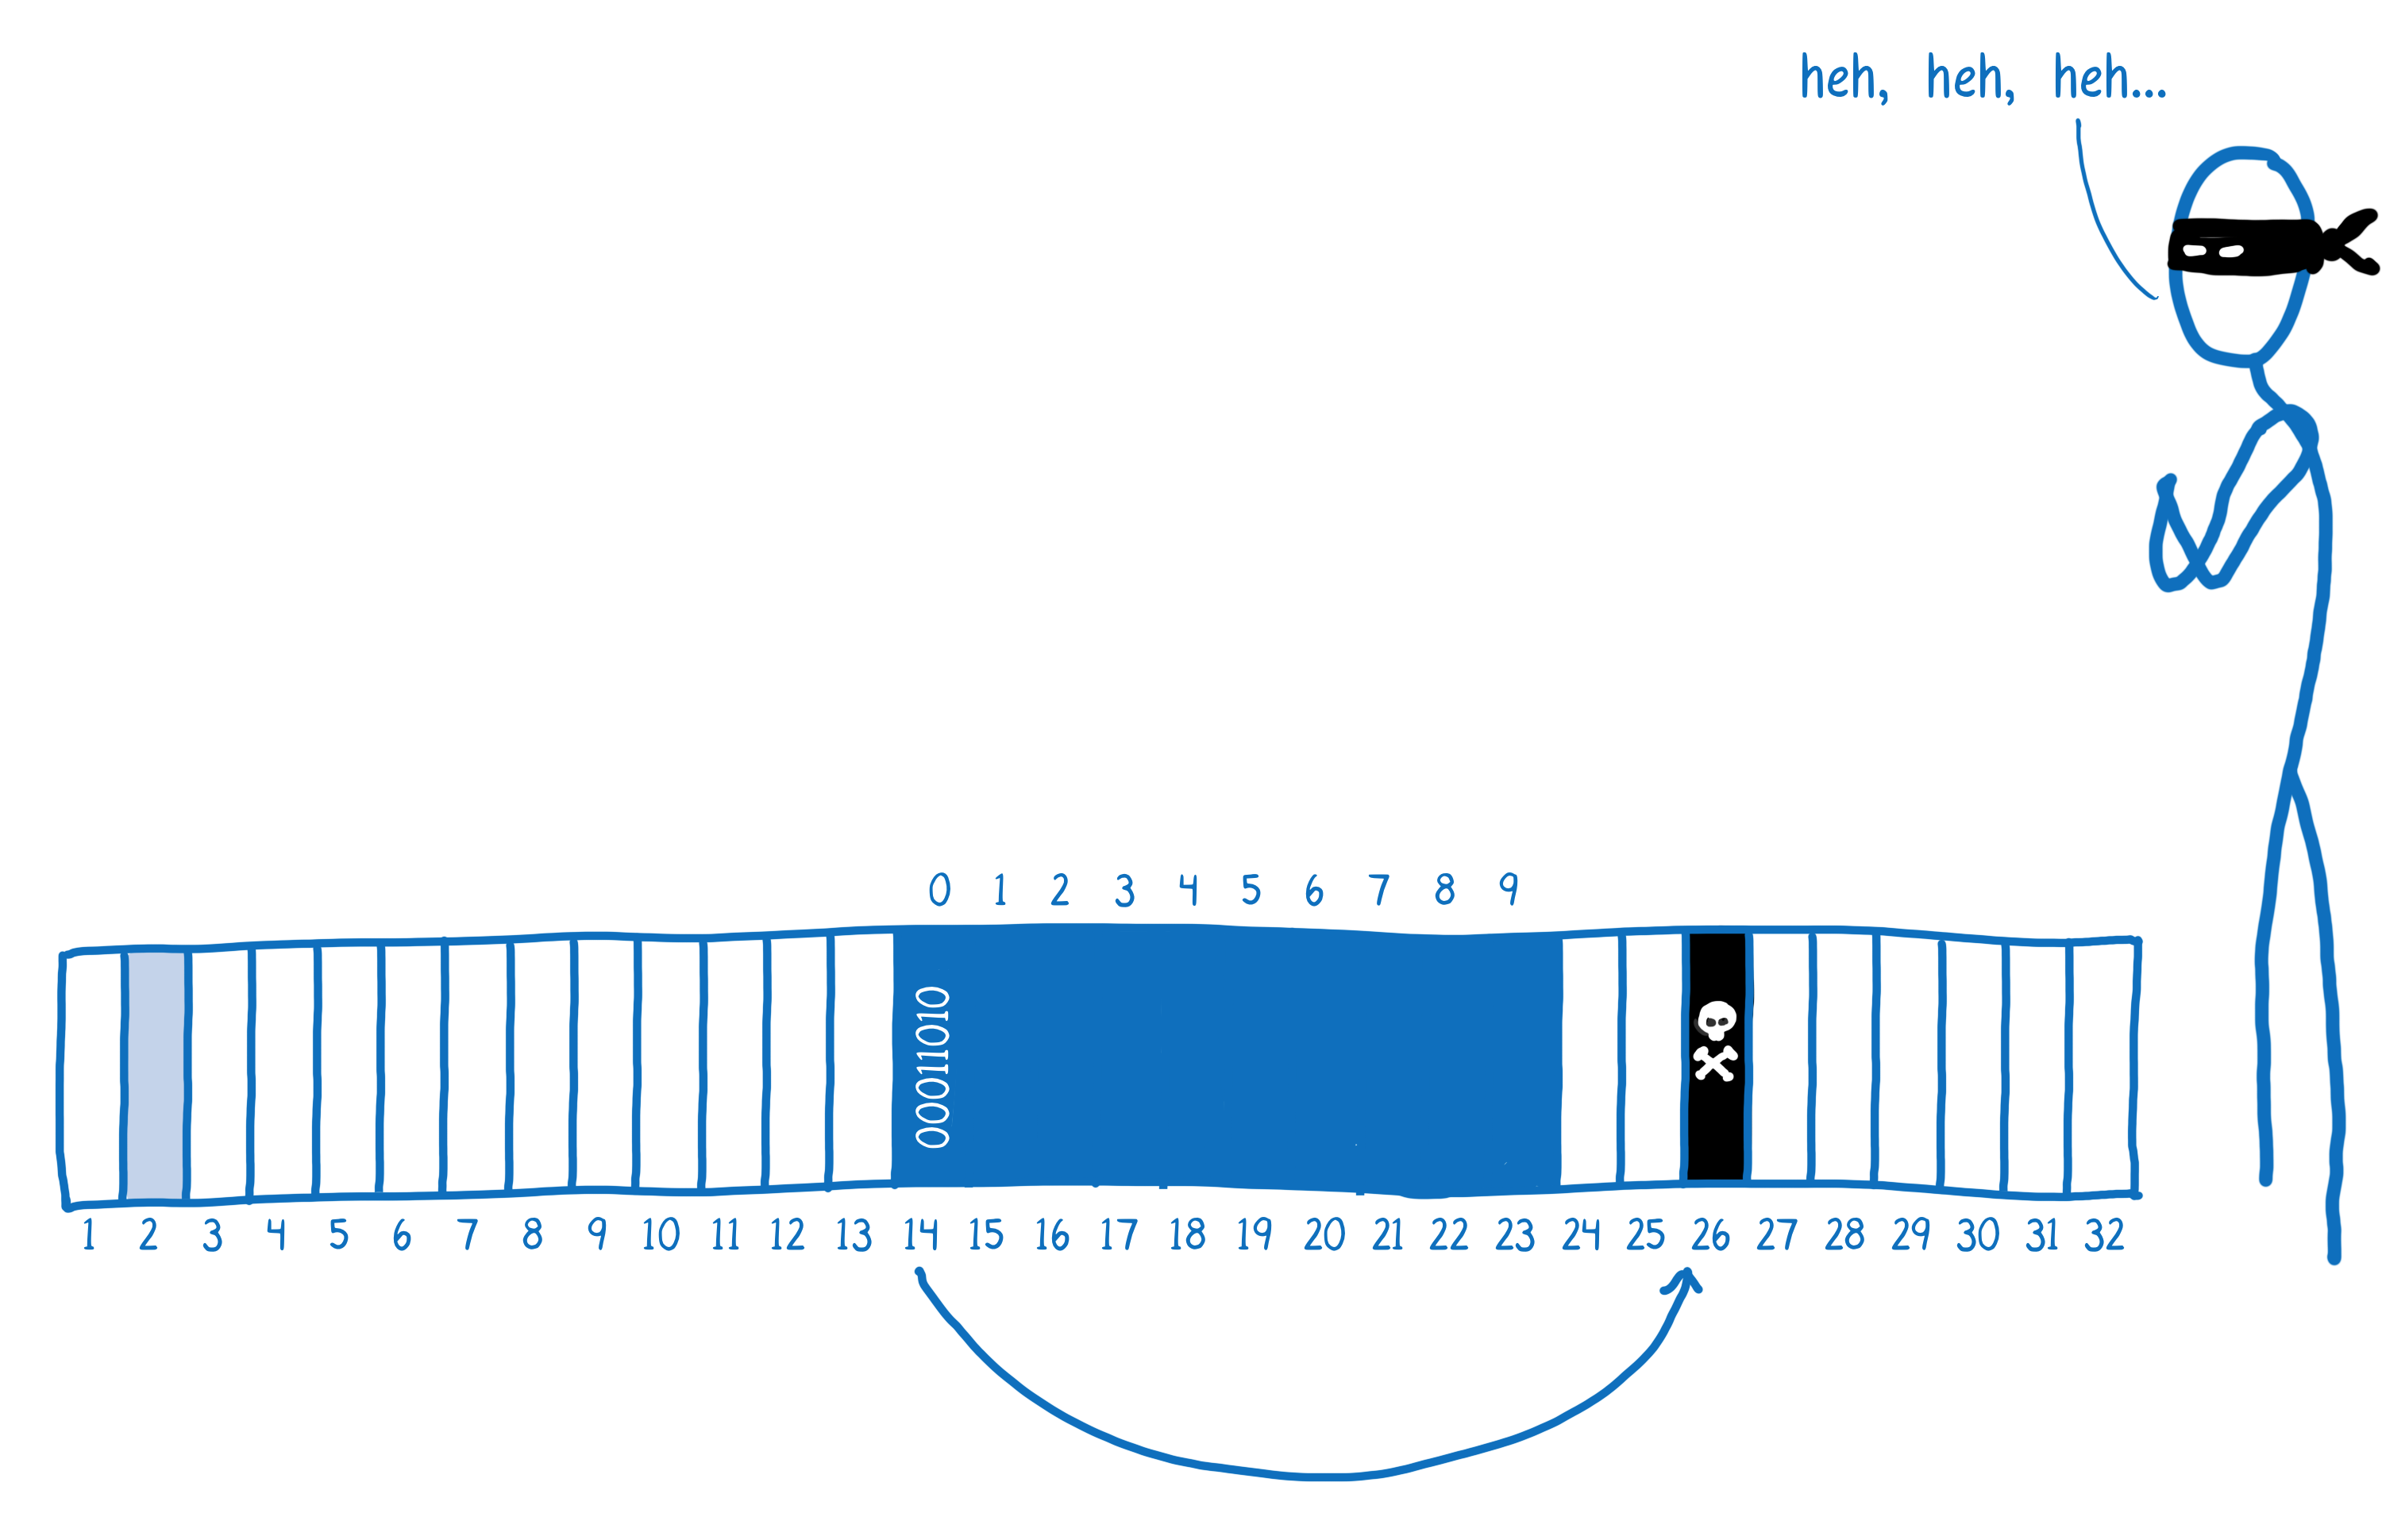
\includegraphics[width=10cm,height=4cm,keepaspectratio]{images/attack.png}}
\end{frame}

\begin{frame}[fragile]
  Rispetto alle mitigazioni include nei binari nativi, la memoria lineare di
  WebAssembly non offre molto dal punto di vista della sicurezza binaria.
\newline\newline
  Cosa succede se si compila un programma \textbf{vulnerabile} in WebAssembly?
\newline\newline
  \begin{minted}{c}
    void vuln() {
      char buffer[16];
      gets(buffer); // !!!
    }
  \end{minted}
\end{frame}

\begin{frame}
  \frametitle{Primitiva di attacco: buffer overflow}
  \begin{columns}
    \begin{column}{0.6\textwidth}
      \begin{itemize}
        \item se la lunghezza dell'input dell'utente non viene controllata,
          è possibile scrivere al di fuori di un buffer
        \begin{itemize}
          \item in particolare è possibile sovrascrivere variabili locali
            all'interno dello stack
        \end{itemize}
        \item l'assenza di mitigazioni nella memoria lineare permette di sovrascrivere dati in altre regioni contigue
        \item funzioni come \textbf{gets()} e \textbf{strcpy()} (senza ulteriori controlli)
          permettono questo tipo di attacco  
      \end{itemize} 
    \end{column}
    \begin{column}{0.4\textwidth}
      \centerline{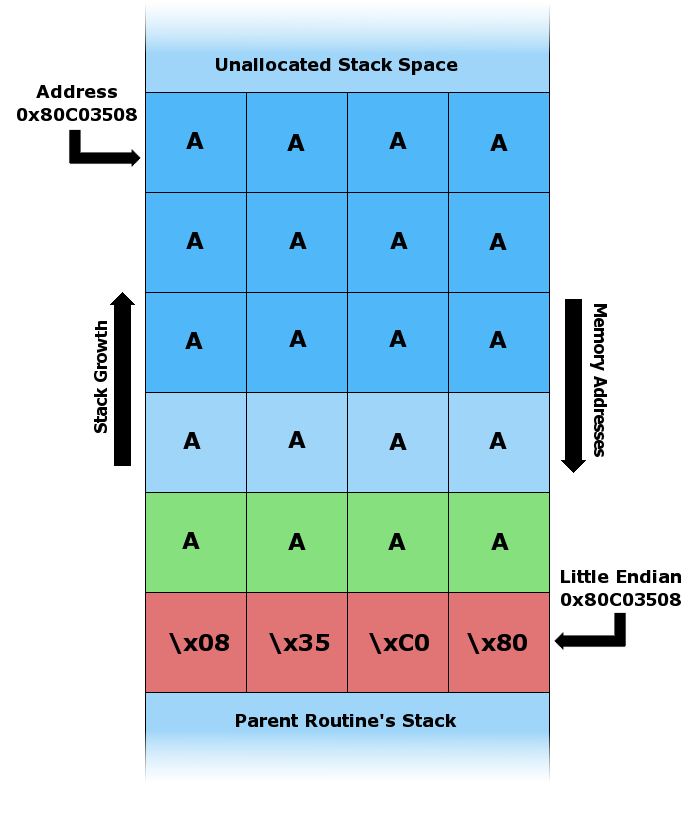
\includegraphics[width=10cm,height=6.5cm,keepaspectratio]{images/stack.png}}
    \end{column}
  \end{columns}
\end{frame}

\begin{frame}[fragile]
  \frametitle{Sovrascrivere dati "costanti"}
  \Fontvi
  \begin{minted}{c}
    char *other_data = "AAAA";

    static char *safe_script = 
      "console.log('this should be safe, shouldn\\'t it?')";


    int main() {
       
      emscripten_run_script(safe_script);
    
    }


    void vuln(const char* input) {
    
      strcpy(other_data, input);

    }
  \end{minted}
\end{frame}

\begin{frame}
  \frametitle{Sovrascrivere dati "costanti"}
  \Fontvi
  \begin{columns}
    \begin{column}{0.55\textwidth}
      \begin{itemize}
        \item le variabili statiche sono salvate nella regione \textbf{data}
        \begin{itemize}
          \item dato che non esistono aree non scrivibili, non esiste una
            sezione dedicata alle variabili costanti (\textbf{.rodata} negli ELF)
        \end{itemize}
      \item \textbf{strcpy()} non effettua controlli sulla dimensioni dell'input
          dell'utente: è possibile sovrascrivere dati sullo stack
        \begin{itemize}
          \item in particolare (con il layout della memoria in figura) un
            overflow nello stack riesce a scrivere nella regione \textbf{data}
        \end{itemize}
        \item sovrascrivendo la stringa puntata dalla variabile safe\_script si
          possono eseguire comandi JavaScript
        \begin{itemize}
          \item \textbf{XSS} nel browser
          \item \textbf{RCE} con Node.js
        \end{itemize}

            \end{itemize}
    \end{column}
    \begin{column}{0.45\textwidth}
      \begin{figure}[htbp]
        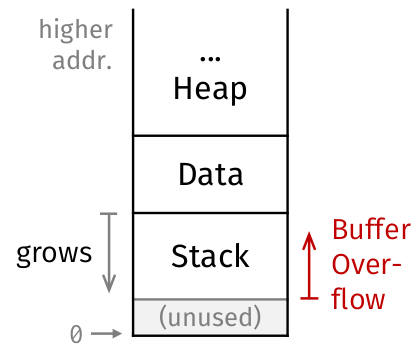
\includegraphics[width=4cm,height=6cm,keepaspectratio]{images/memory_layout.png}
        \newline\newline\newline
        \begin{figure}
          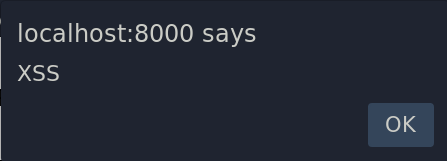
\includegraphics[width=4cm,height=6cm,keepaspectratio]{images/xss.png}
          \caption{Chiamando \textbf{vuln()} con la stringa
          ";;;;;;;;;;;;;;;;;;;;;;;;;;;;;;;;;alert('XSS')"}
        \end{figure}
        \end{figure}
    \end{column}
  \end{columns}
\end{frame}

\begin{frame}[fragile]
  \frametitle{Sovrascrivere dati sullo heap}
  \begin{itemize}
    \item similmente è possibile sovrascrivere stringhe sullo heap
    \item la libreria \textbf{libpng} contiene un buffer overflow che
      è possibile sfruttrare convertendo un immagine da pnm a png 
  \end{itemize}
  \begin{minted}{c++}
    int main() {
      std::string img_tag = 
        "<img src='data:image/png;base64,";
      // CVE-2018-14550
      pnm2png("input.pnm", "output.png");        
      img_tag += file_to_base64("output.png") + "'>";
      emcc::global("document").call("write", img_tag);
    }
  \end{minted}
  \begin{itemize}
    \item se l'input dell'utente non viene controllato/sanitizzato, è possibile
      sovrascrivere la string \textbf{img\_tag} situata nello heap 
    \item questo causa un attacco di tipo XSS nel browser
  \end{itemize}
\end{frame}

\begin{frame}
  \frametitle{Sovrascrivere dati sullo heap}
  \Fontvi 
  \begin{columns}
    \begin{column}{0.5\textwidth}
      \begin{figure}
        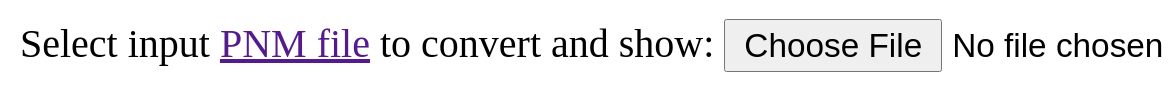
\includegraphics[width=5cm,height=6cm,keepaspectratio]{images/site.png}
        \caption{Il sito chiede all'utente un'immagine in input: non vengono
        fatti controlli sul tipo di file} 
      \end{figure} 
      \begin{figure}
        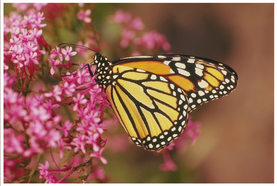
\includegraphics[width=4cm,height=4cm,keepaspectratio]{images/butfly.png}
        \caption{Se l'utente immette un'immagine, questa viene convertita
        e mostrata nel browser} 
      \end{figure} 

    \end{column}
    \begin{column}{0.5\textwidth}
      Utilizzando come payload
      \newline\newline\newline
      AAAAAAAAAAAAAAAAAAAAAAAA...
      <script>alert('XSS')</script><!- -
      \newline\newline\newline
      è possibile sovrascrivere i dati nello stack (con una sequenza specifica di A) e sostituire al tag
      \textbf{<img>} il tag \textbf{<script>} nello heap: questo provoca un attacco di
      tipo XSS
      \newline\newline\newline
      \centerline{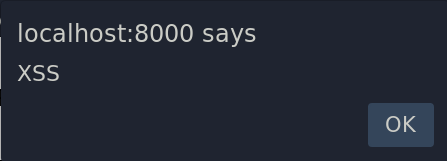
\includegraphics[width=5.5cm,height=5.5cm,keepaspectratio]{images/xss.png}}
    \end{column}

  \end{columns}
\end{frame}


\begin{frame}
  \frametitle{Conclusioni}
  \begin{itemize}
    \item WebAssembly ha reintrodotto vulnerabilitá precendentemente mitigate
      e introdotto nuovi tipi di attacchi, come sovrascivere dati costanti
    \item  
  \end{itemize}
\end{frame}

\begin{frame}
  \frametitle{Bibliografia}
  \begin{enumerate}
    \item Daniel Lehmann, Johannes Kinder, Michael Pradel: \emph{"Everything Old is New Again:
      Binary Security of WebAssembly"}
    \item Brian McFadden, Tyler Lukasiewicz, Jeff Dileo, Justin Engler:
      \emph{"Security Chasms of WASM"}
  \end{enumerate}
\end{frame}

\end{document}
